% Copyright 2004 by Till Tantau <tantau@users.sourceforge.net>.
%
% In principle, this file can be redistributed and/or modified under
% the terms of the GNU Public License, version 2.
%
% However, this file is supposed to be a template to be modified
% for your own needs. For this reason, if you use this file as a
% template and not specifically distribute it as part of a another
% package/program, I grant the extra permission to freely copy and
% modify this file as you see fit and even to delete this copyright
% notice. 

\documentclass{beamer}

% There are many different themes available for Beamer. A comprehensive
% list with examples is given here:
% http://deic.uab.es/~iblanes/beamer_gallery/index_by_theme.html
% You can uncomment the themes below if you would like to use a different
% one:
%\usetheme{AnnArbor}
%\usetheme{Antibes}
%\usetheme{Bergen}
%\usetheme{Berkeley}
%\usetheme{Berlin}
%\usetheme{Boadilla}
%\usetheme{boxes}
%\usetheme{CambridgeUS}
%\usetheme{Copenhagen}
%\usetheme{Darmstadt}
%\usetheme{default}
%\usetheme{Frankfurt}
%\usetheme{Goettingen}
%\usetheme{Hannover}
%\usetheme{Ilmenau}
%\usetheme{JuanLesPins}
%\usetheme{Luebeck}
%\usetheme{Madrid}
%\usetheme{Malmoe}
%\usetheme{Marburg}
%\usetheme{Montpellier}
%\usetheme{PaloAlto}
%\usetheme{Pittsburgh}
%\usetheme{Rochester}
%\usetheme{Singapore}
%\usetheme{Szeged}
%\usetheme{Warsaw}

\usepackage{amsmath}
\usepackage{textpos}
\usepackage{ulem}
%\usepackage{enumitem}
\usepackage{bm}
\usepackage{algorithm}
\usepackage[noend]{algpseudocode}
\usepackage{subfigure}

\usepackage{amsthm}
\newtheorem{thm}{Theorem}

\usepackage{paralist}
\usepackage{comment} 

\usepackage[labelformat=empty]{caption}

\definecolor{BYUblue}{RGB}{0,31,69}
\definecolor{BYUgold}{RGB}{195,163,106}
\usecolortheme[RGB={0,31,69}]{structure} % BYU Blue

\definecolor{diff-point}{RGB}{102,178,255}
\definecolor{diff-path}{RGB}{0,76,153}

\definecolor{reference_color}{RGB}{0,175,0}
\definecolor{subproblem_color}{RGB}{0,0,255}

\newtheorem{reference_tree}{Example}
\newtheorem{subproblem_tree}{Example}
\newenvironment<>{reference_tree}[1][]{%
  \setbeamercolor{block title example}{fg=white,bg=reference_color}%
  \begin{example}#2[#1]}{\end{example}}
\newenvironment<>{subproblem_tree}[1][]{%
  \setbeamercolor{block title example}{fg=white,bg=subproblem_color}%
  \begin{example}#2[#1]}{\end{example}}


\usetheme{Frankfurt}
\setbeamercolor*{section in head/foot}{bg=BYUblue,fg=gray!25}
\setbeamercolor*{frametitle}{bg=BYUblue!50,fg=white!25}
\setbeamercovered{transparent}
\mode<all>

\DeclareMathOperator*{\argmax}{arg\,max}

\title{From Qualitative to Quantitative: Supporting Robot Understanding in Human-Interactive Path Planning}

\subtitle{\bf [ Research Area ] }

\author{Daqing Yi
}

\institute
{
  Department of Computer Science\\
  Brigham Young University
}

\date[]{} 

\addtobeamertemplate{frametitle}{}{%
\begin{textblock*}{100mm}(0.9\textwidth,-1.2cm)

\includegraphics[width=1.1cm]{figure/BYU_logo.png}
\end{textblock*}}

\begin{document}

\begin{frame}
  \titlepage
\end{frame}

\begin{frame}{Outline}{$ \null $}
  \tableofcontents
  % You might wish to add the option [pausesections]
\end{frame}

% Section and subsections will appear in the presentation overview
% and table of contents.

% Add citation in the footnote

\section{Motivation}

% add outline page with current section highlighted.
\begin{frame}{Outline}{ $ \null $ }
	\tableofcontents[currentsection]
	%\tableofcontents[currentsection,currentsubsection]
\end{frame}

\subsection{Differences between Human and Robot}

\begin{frame}{Humans and Robots Think Differently}{Motivation}

\begin{columns}
\column{0.4\textwidth}
\begin{block}{ Human's Brain }
\centering
{\bf Krang}
\begin{figure}
	\centering
	
\includegraphics[width=.7\linewidth]{figure/human_brain}
\end{figure}
\end{block}	
\column{0.4\textwidth}
\begin{block}{ Robot's Chip }
\centering
{\bf Baymax}
\begin{figure}
	\centering
	
\includegraphics[width=.7\linewidth]{figure/baymax_and_chip}
\end{figure}
\end{block}	
\end{columns}

\end{frame}

\begin{frame}{Qualitative vs Quantitative}{Motivation}

\begin{block}{}

Humans and robots process and express in different way.

\end{block}

\begin{columns}
\column{0.47\textwidth}

\begin{block}{ Qualitative }

\begin{minipage}[t][5cm][t]{.9\textwidth}

\centering
{\bf ``I am at the east of the TMCB.''}

\begin{figure}
	\centering
	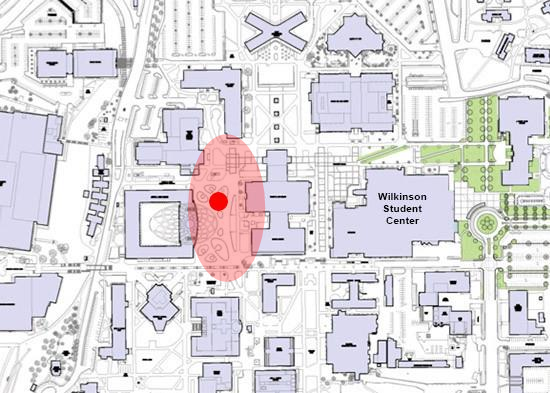
\includegraphics[width=\linewidth]{figure/human_localization_rough}
\end{figure}
\end{minipage}

\end{block}

\column{0.47\textwidth}

\begin{block}{ Quantitative }

\begin{minipage}[t][5cm][t]{.9\textwidth}

\centering
{\bf Location $( 35.7 , 47.5 )$ \\ Orientation 72.1$^{\circ}$}

\begin{figure}
	\centering
	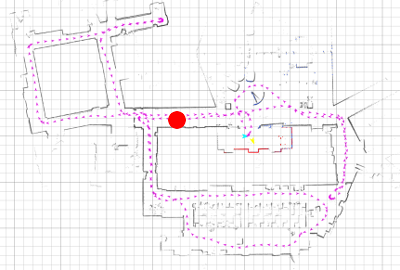
\includegraphics[width=\linewidth]{figure/robot_localization}
\end{figure}
\end{minipage}

\end{block}

\end{columns}

\end{frame}

\begin{frame}{Qualitative vs Quantitative}{Motivation}

\begin{columns}
\column{0.47\textwidth}

\begin{block}{ Qualitative }

\begin{minipage}[t][5cm][t]{.9\textwidth}

\centering
{\bf ``An apple is good, and a banana is better.''}

\begin{figure}
	\centering
	
\includegraphics[width=.45\linewidth]{figure/human_preference}
\end{figure}
\end{minipage}

\end{block}

\column{0.47\textwidth}

\begin{block}{ Quantitative }

\begin{minipage}[t][5cm][t]{.9\textwidth}

\centering
{\bf {\sc \bf Utility}( banana ) $ = 100 $ \\ {\sc \bf Utility}( apple ) $ = 80 $ }

\begin{figure}
	\centering
	
\includegraphics[width=.6\linewidth]{figure/robot_preference}
\end{figure}
\end{minipage}

\end{block}

\end{columns}

\end{frame}

\begin{frame}{Human-Robot Collaboration}{Motivation}

\begin{columns}
\column{0.4\textwidth}
\begin{block}{ Human's Role }
\begin{minipage}[t][1.2cm][t]{.9\textwidth}
\centering
\begin{itemize}
\item {\bf Coach}
\item {\bf Player}
\end{itemize}
\end{minipage}
\end{block}	
\column{0.4\textwidth}
\begin{block}{ Robot's Role }
\begin{minipage}[t][1.2cm][t]{.9\textwidth}
\centering
\begin{itemize}
\item {\bf Player}
\end{itemize}
\end{minipage}
\end{block}	
\end{columns}

\begin{figure}
	\centering
	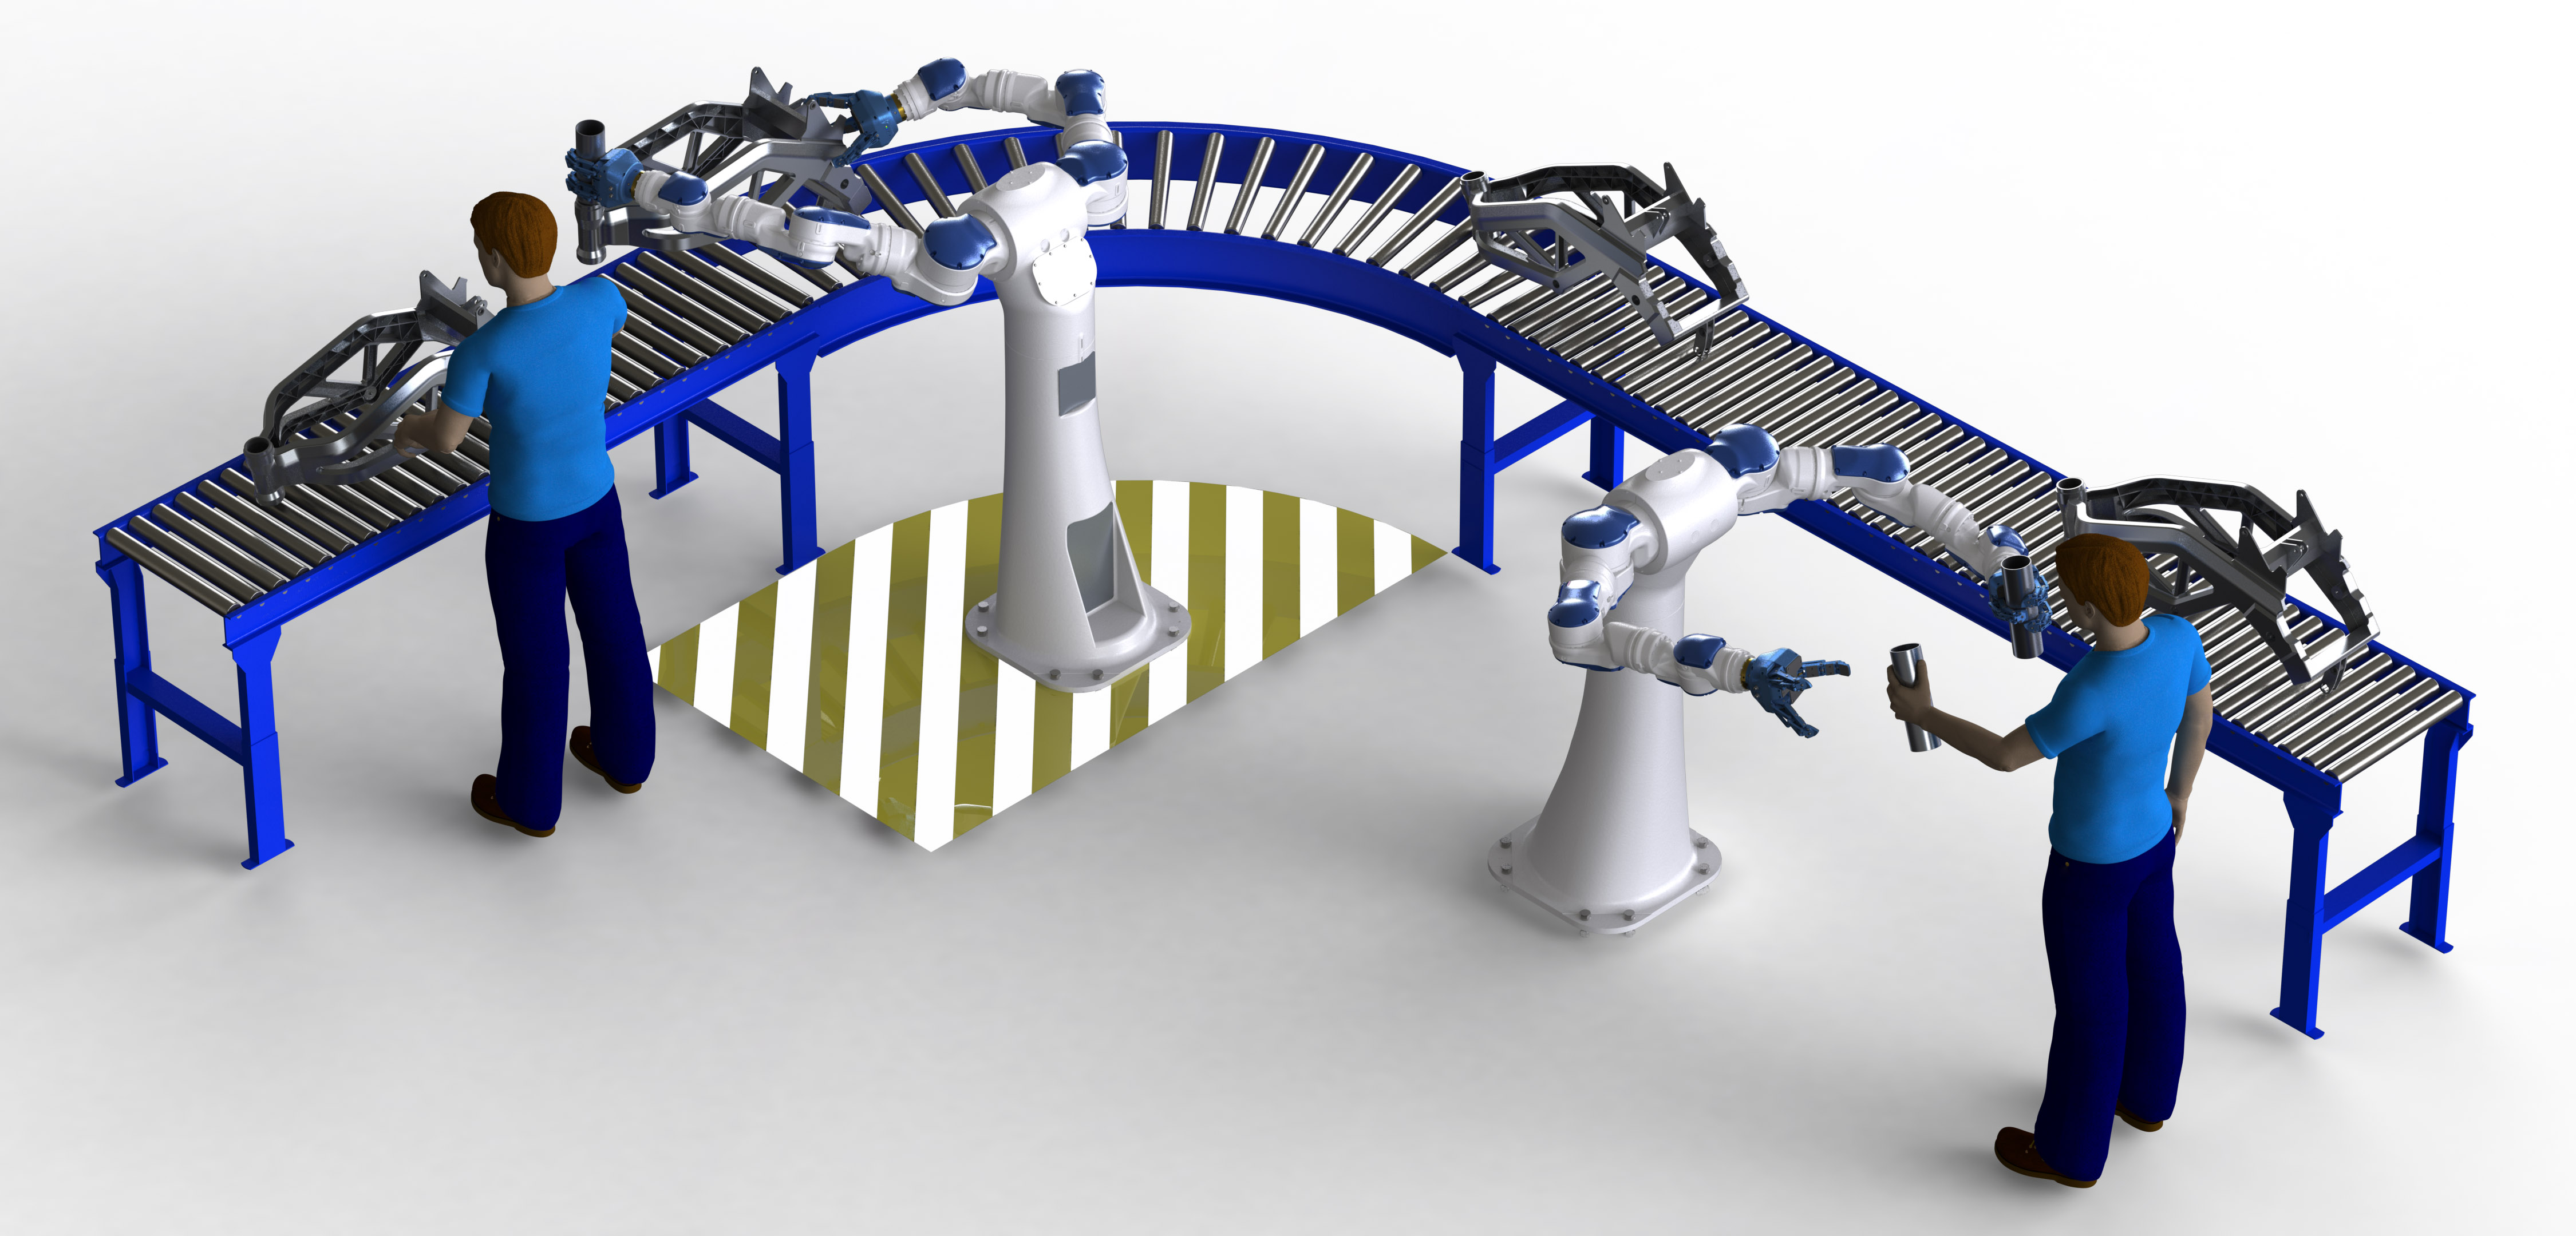
\includegraphics[width=.7\linewidth]{figure/human_robot_collaboration}
\end{figure}

\end{frame}

\begin{frame}{Human-Robot Collaboration}{Motivation}

\begin{figure}
	\centering
	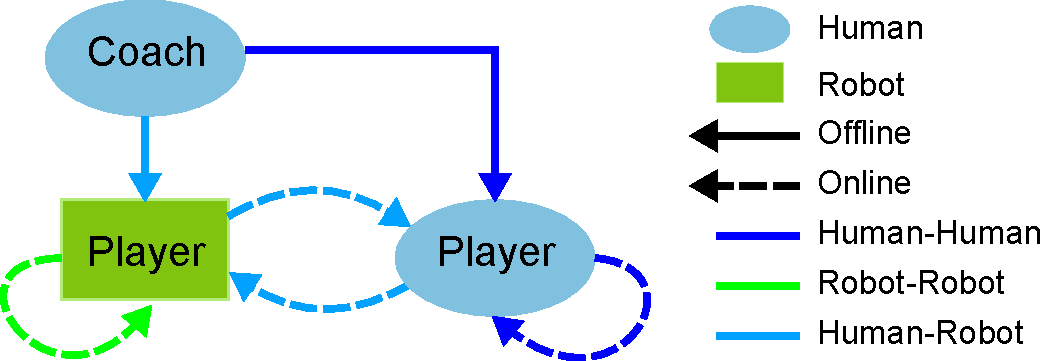
\includegraphics[width=.7\linewidth]{figure/team_info_flow}
\end{figure}

\end{frame}

\begin{frame}{From Quantitative to Qualitative}{Motivation}

\begin{columns}
\column{0.45\textwidth}
\begin{block}{ Location }
\begin{minipage}[t][4cm][t]{\textwidth}
\centering

\begin{itemize}
\item softmax regression
\end{itemize}
\begin{figure}
	\centering
	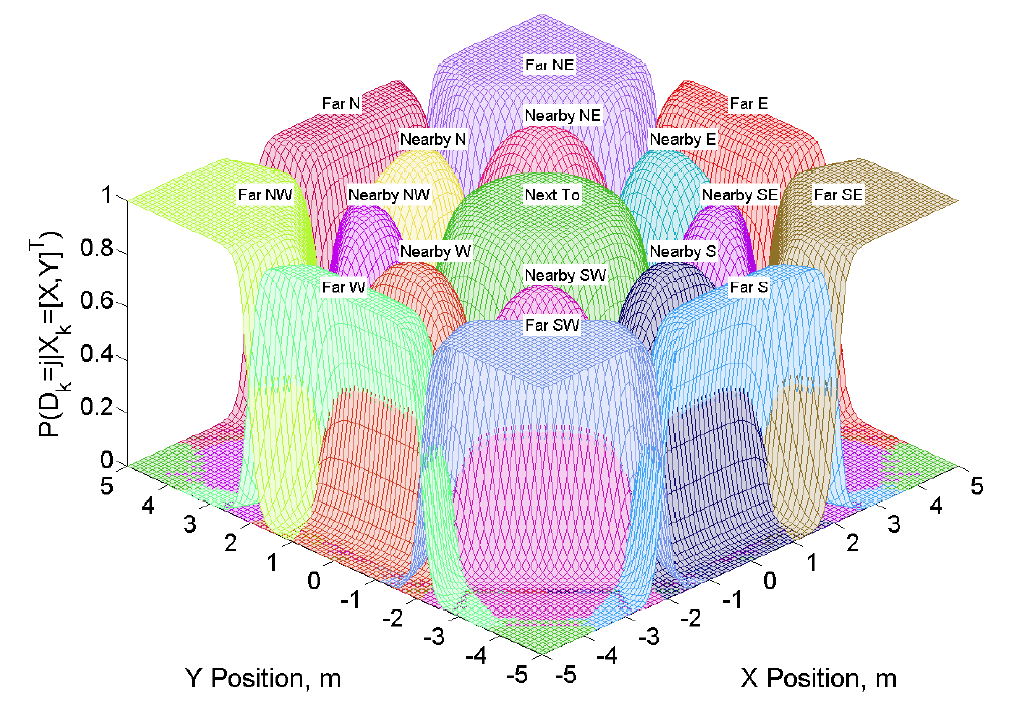
\includegraphics[width=.9\linewidth]{figure/softmax_func}
	\caption{ \tiny{ {\it Sample et al.} "An experimental evaluation of Bayesian soft human sensor fusion in robotic systems."  2012 AIAA Guidance, Navigation and Control Conference.} }
\end{figure}

\end{minipage}
\end{block}	
\column{0.45\textwidth}
\begin{block}{ Preference }
\begin{minipage}[t][4cm][t]{\textwidth}
\centering

\begin{itemize}
\item fuzzy membership function
\end{itemize}
\begin{figure}
	\centering
	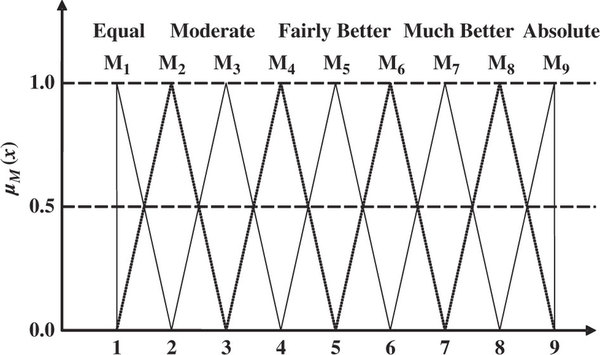
\includegraphics[width=.9\linewidth]{figure/membership_func}
	\caption{ \tiny{ {\it Wang et al. } ``A comprehensive decision support model for the evaluation of eco-designs.'' Journal of the Operational Research Society 2013. } }
\end{figure}

\end{minipage}
\end{block}	
\end{columns}

\end{frame}

\begin{frame}{From Qualitative to Quantitative?}{Motivation}

\begin{columns}
\column{0.4\textwidth}
\begin{minipage}[t]{.9\textwidth}
\begin{block}{ Location }
\centering
\begin{figure}
	\centering
	
\includegraphics[width=.4\linewidth]{figure/question_mark}
\end{figure}
\end{block}
\end{minipage}
\column{0.4\textwidth}
\begin{minipage}[t]{.9\textwidth}
\begin{block}{ Preference }
\centering
\begin{figure}
	\centering
	
\includegraphics[width=.4\linewidth]{figure/question_mark}
\end{figure}
\end{block}
\end{minipage}	
\end{columns}

\begin{block}{\bf Approach}

\begin{center}
\begin{minipage}[t]{.8\textwidth}
\begin{block}{}
\begin{itemize}
\item Probabilistic model
\end{itemize}
\end{block}
\end{minipage}
\end{center}

\begin{center}
\begin{minipage}[t]{.8\textwidth}
\centering
\begin{block}{}
\begin{itemize}
\item Posterior method
\end{itemize}
\end{block}
\end{minipage}
\end{center}

\end{block}

\end{frame}




\section{Path Planning}

\begin{frame}{Informative Path Planning}{Information measurement}
\begin{itemize}
\item minimize the uncertainty of the observed environment
\end{itemize}
\begin{figure}
	\centering
	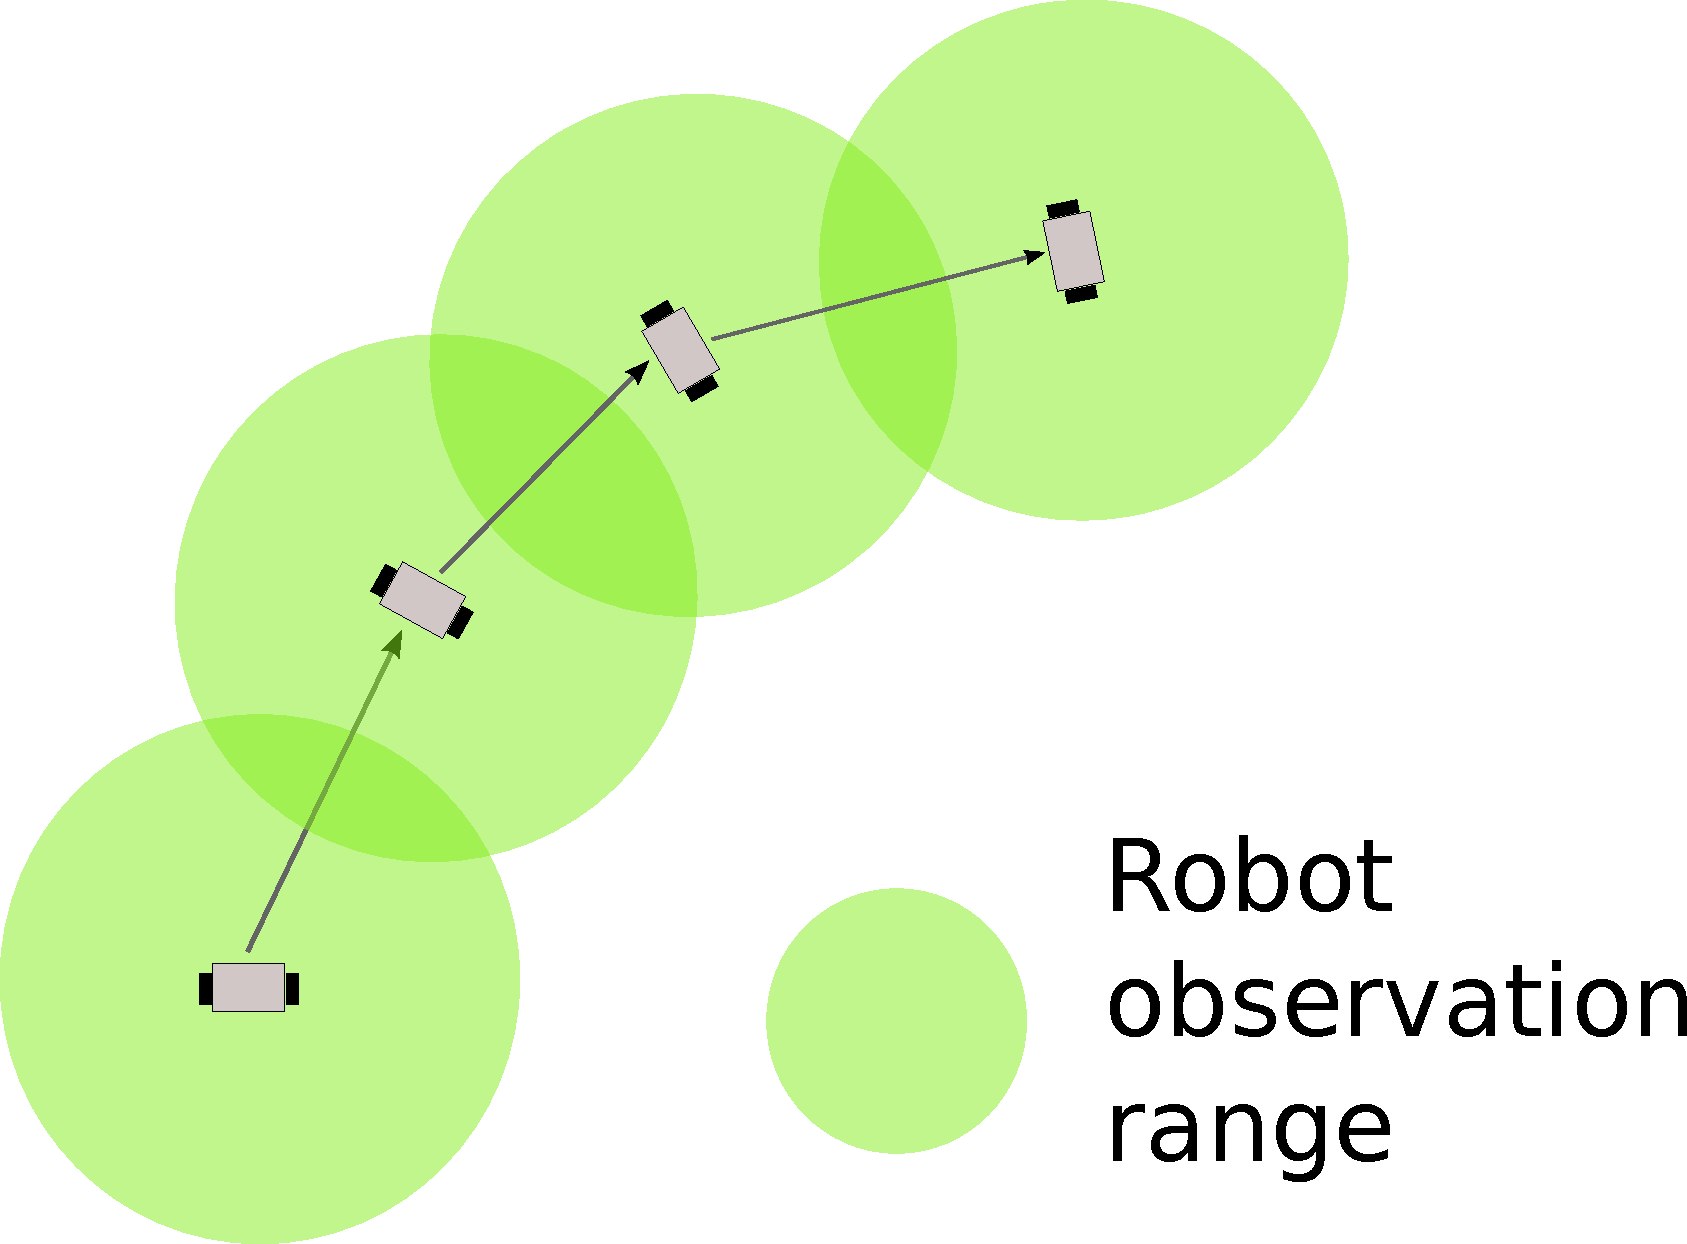
\includegraphics[width = .6\textwidth]{./figure/robotObservation}
\end{figure}
\end{frame}

\begin{frame}{Cordon and search}{Application}
\begin{columns}
	\column{0.5\textwidth}
	\begin{minipage}{\textwidth}
		\begin{figure}
			\centering
			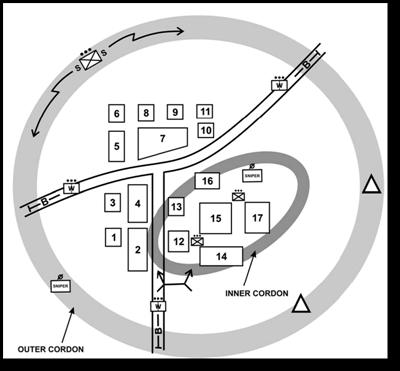
\includegraphics[width = 0.9\textwidth]{./figure/cordon_and_search.jpg}
		\end{figure}
	\end{minipage}
	
	\column{0.5\textwidth}
	\begin{minipage}{\textwidth}
		\begin{figure}
			\centering
			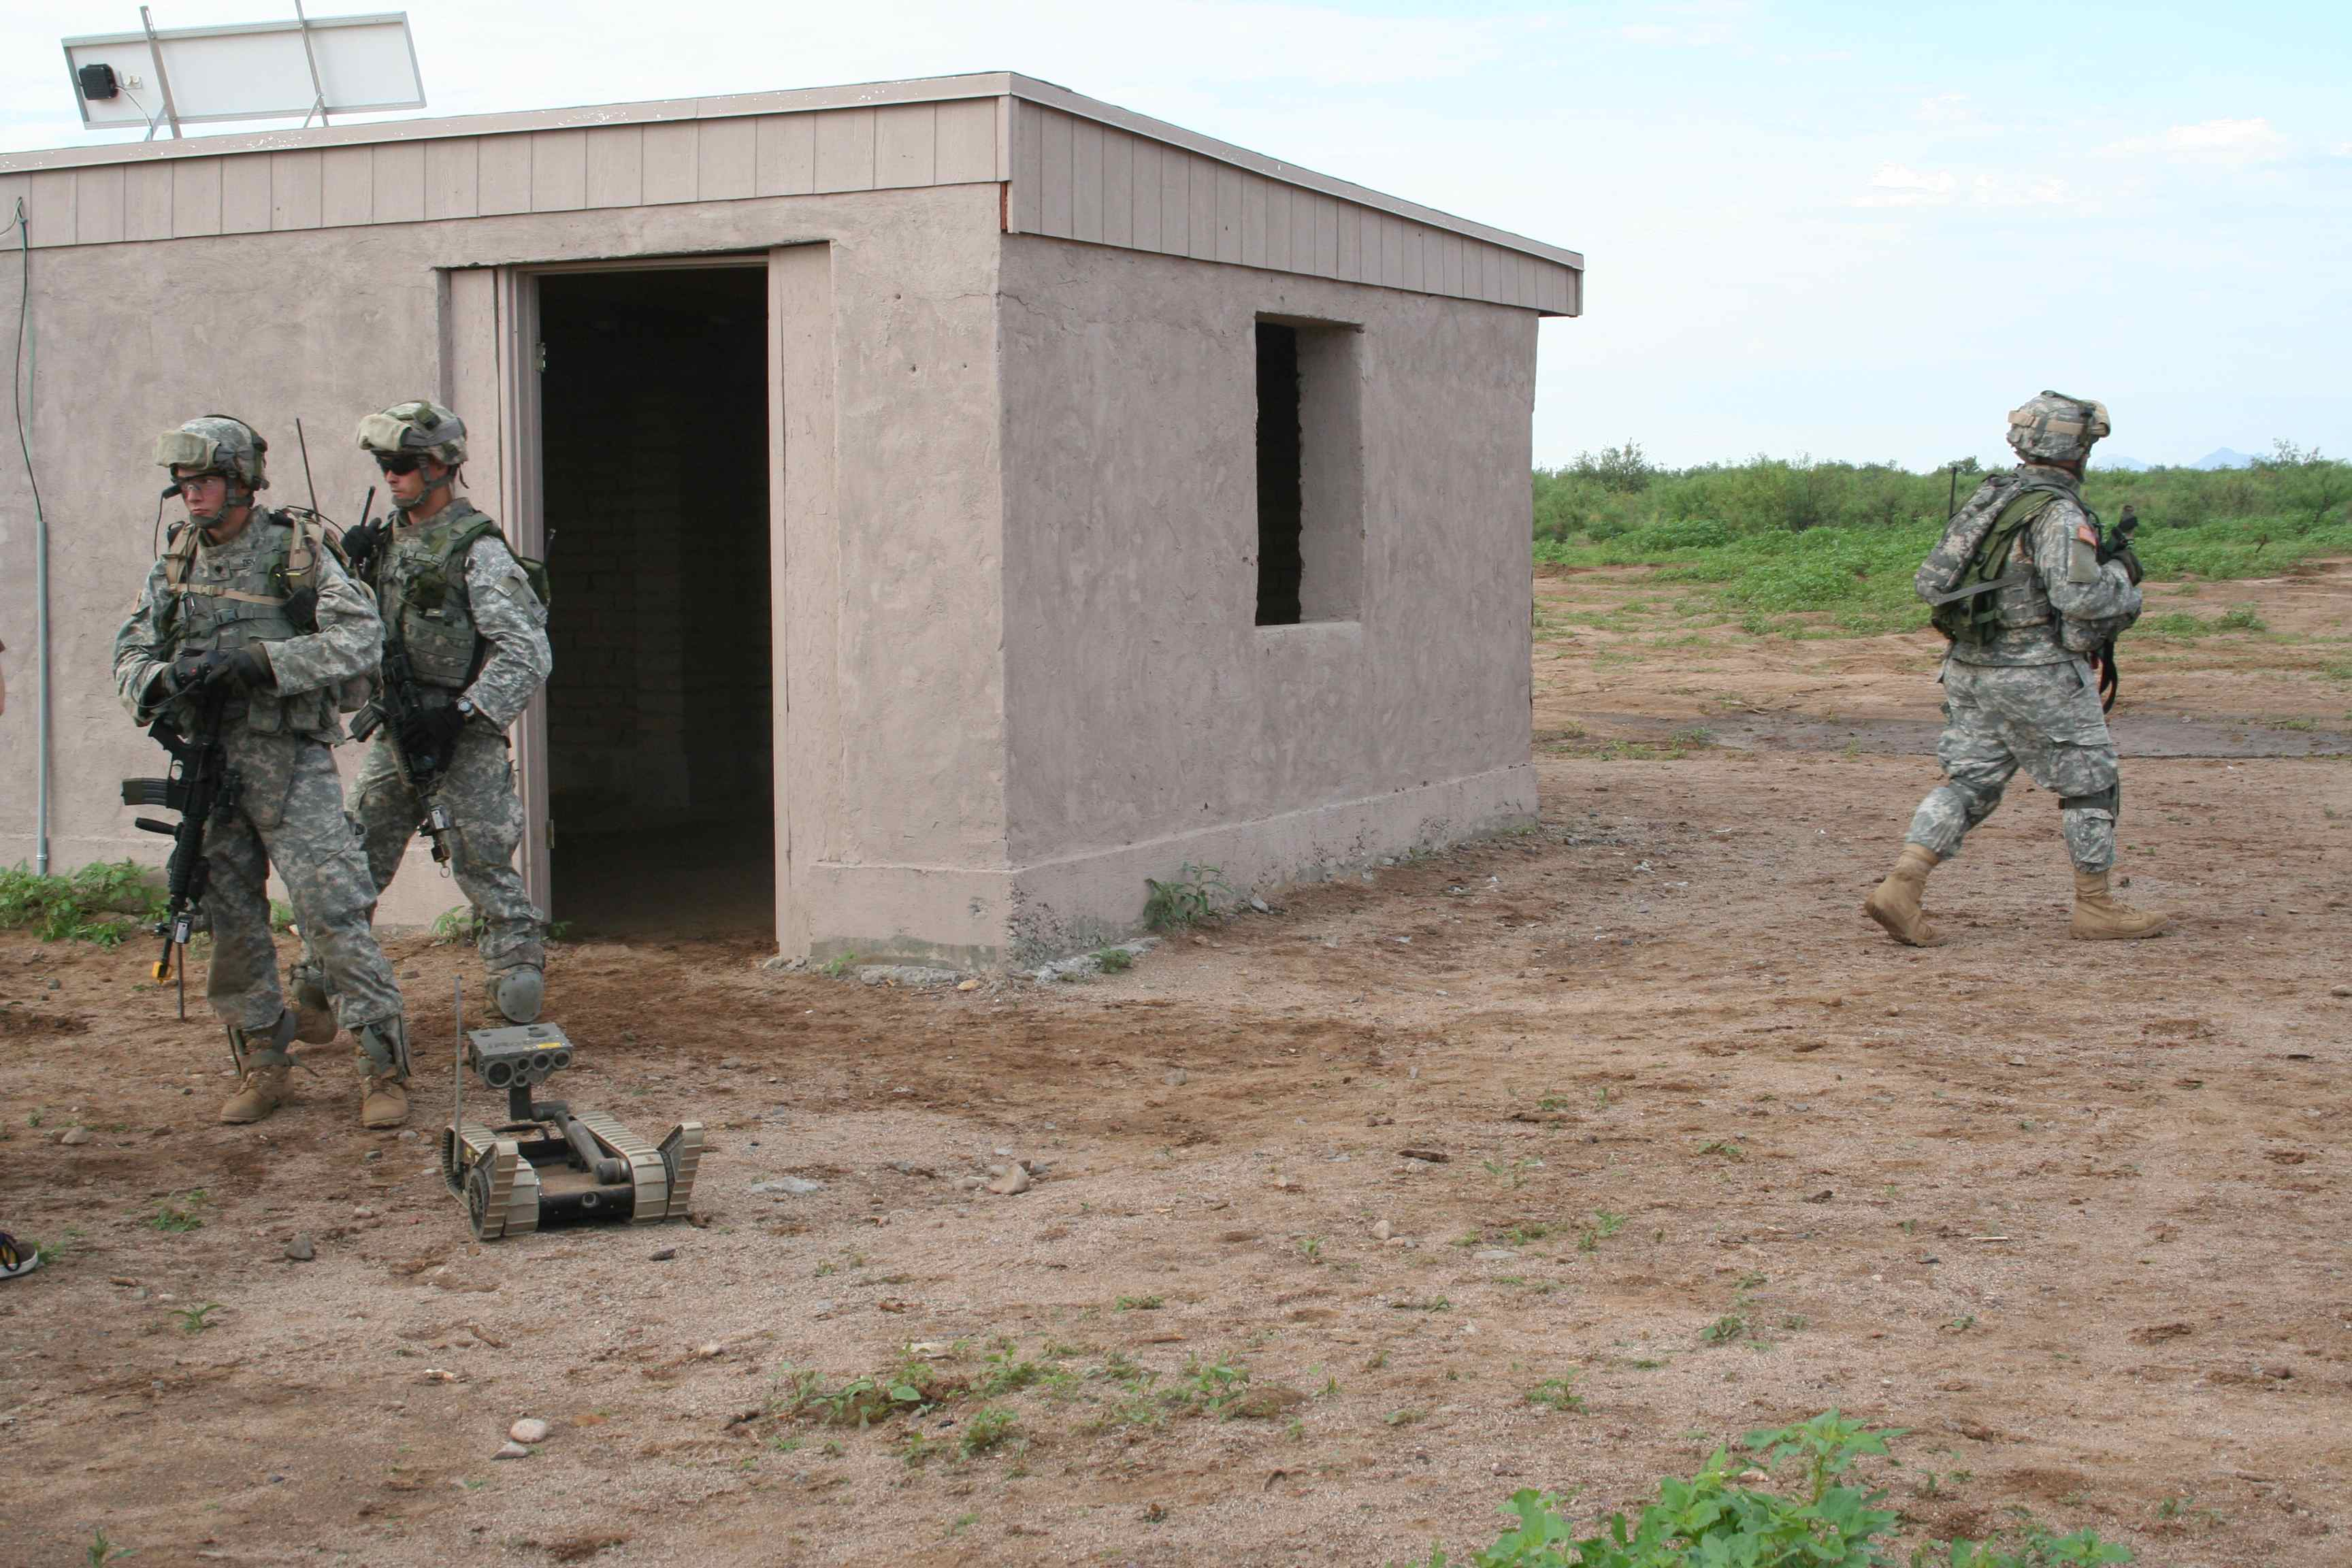
\includegraphics[width = 0.9\textwidth]{./figure/soldier_and_robot.jpg}
		\end{figure}
	\end{minipage}	
\end{columns}
\end{frame}

\begin{frame}{Map discretization}{Application}
	\begin{columns}
		\column{0.5\textwidth}
		\begin{minipage}{\textwidth}
			\begin{figure}
				\centering
				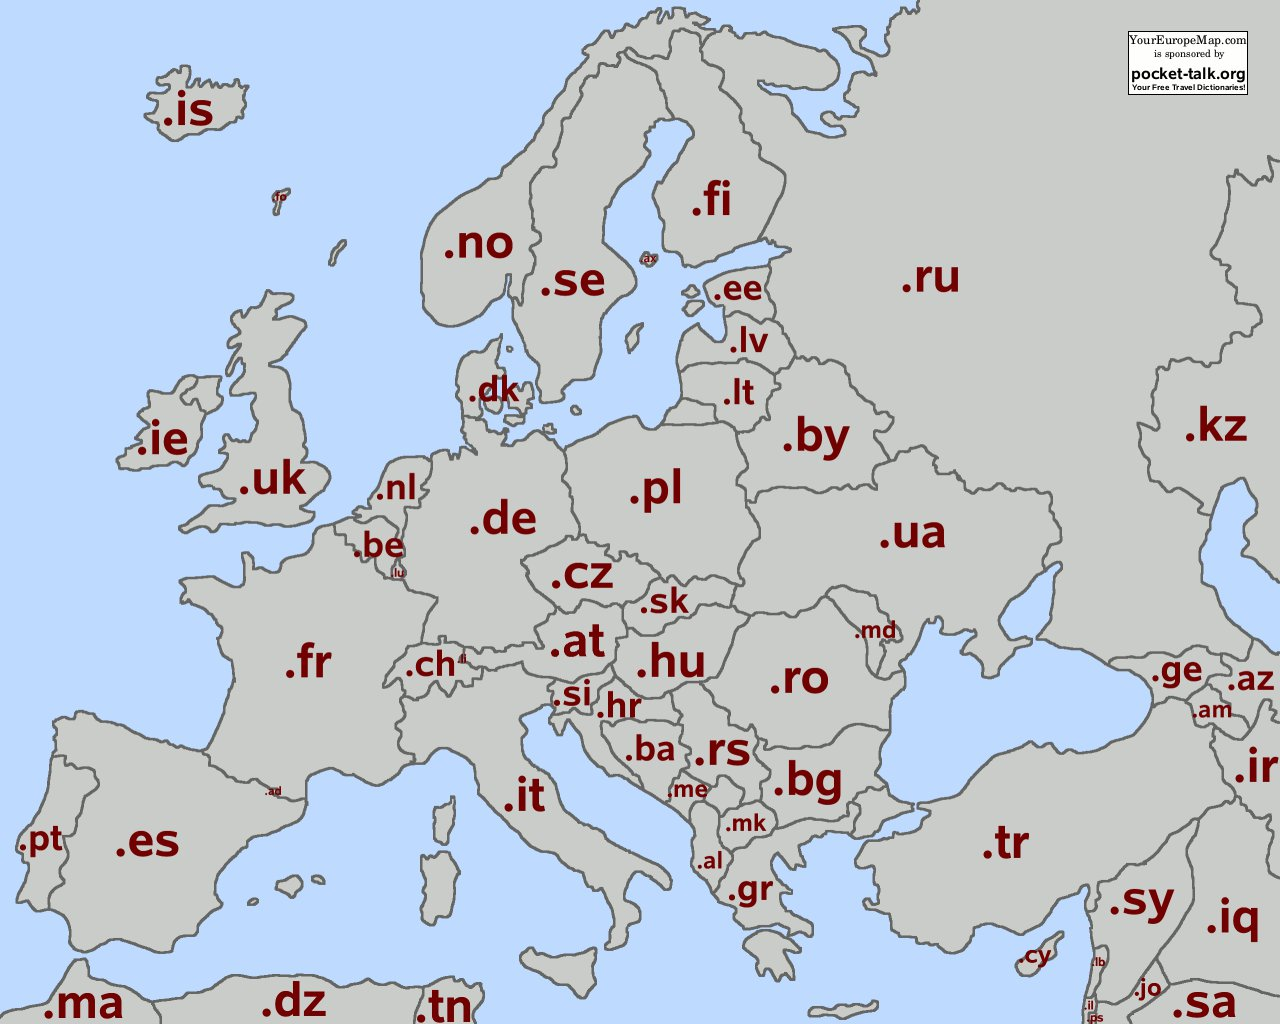
\includegraphics[width = 0.9\textwidth]{./figure/map_tld_europe.jpg}
			\end{figure}
		\end{minipage}
		
		\column{0.5\textwidth}
		\begin{minipage}{\textwidth}
			\begin{figure}
				\centering
				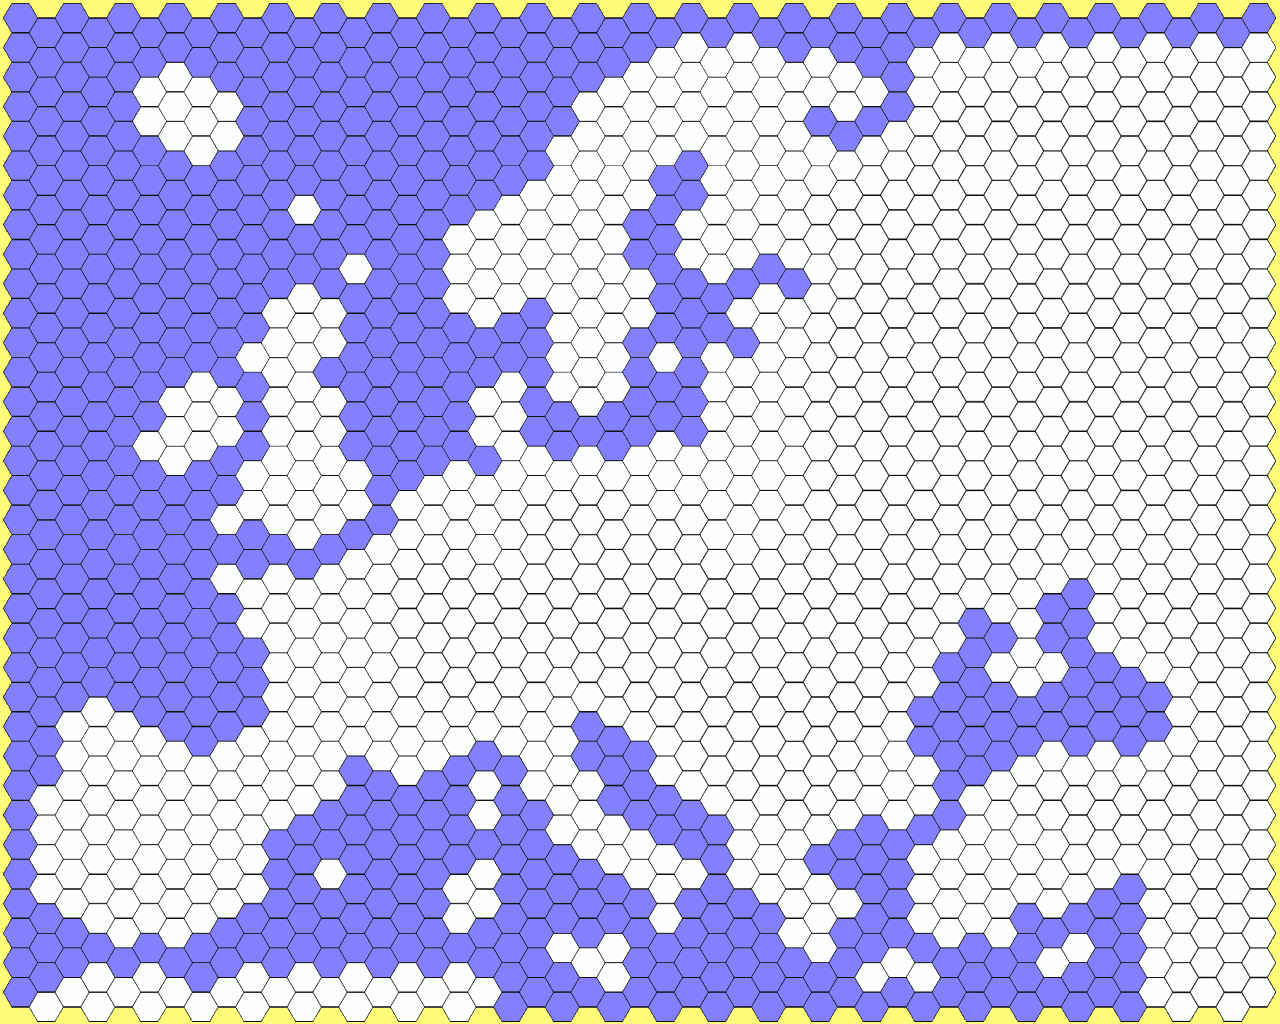
\includegraphics[width = 0.9\textwidth]{./figure/hexagonal_europe_map.png}
			\end{figure}
		\end{minipage}	
	\end{columns}
\end{frame}

\begin{frame}{Submodular orienteering}{Informative path}
	\begin{itemize}
	\item $ \mathbf{S} $ - Environment states
	\item $ \mathbf{O}^{X} $ - Robot's observations
	\item $ \mathbf{O}^{Y^{h}} $ - Human's obeservations
	\end{itemize}
	\begin{block}{Conditional mutual information}
		$ I(\mathbf{S}; \mathbf{O}^{X} \mid \mathbf{O}^{Y^{h}}) = H(\mathbf{S} \mid \mathbf{O}^{Y^{h}}) - H(\mathbf{S} \mid \mathbf{O}^{X},\mathbf{O}^{Y^{h}}) $
	\end{block} 
	
	\bigskip
	
	\begin{itemize}
		\item Entropy reduction
		\item Submodularity
		\item Chain rule \\
		$ I(\mathbf{S}; \mathbf{O}^{X} \mid \mathbf{O}^{Y^{h}}) = \sum_{t=1}^{T} I(O^{X}_{t} ; \mathbf{S} \mid O^{X}_{1} , \cdots , O^{X}_{t-1}, \mathbf{O}^{Y^{h}}) $
	\end{itemize}
	
\end{frame}

%\subsection{Human constraint}

\begin{frame}{Team role}{Human constraint}
	
	\begin{figure}
		\centering
		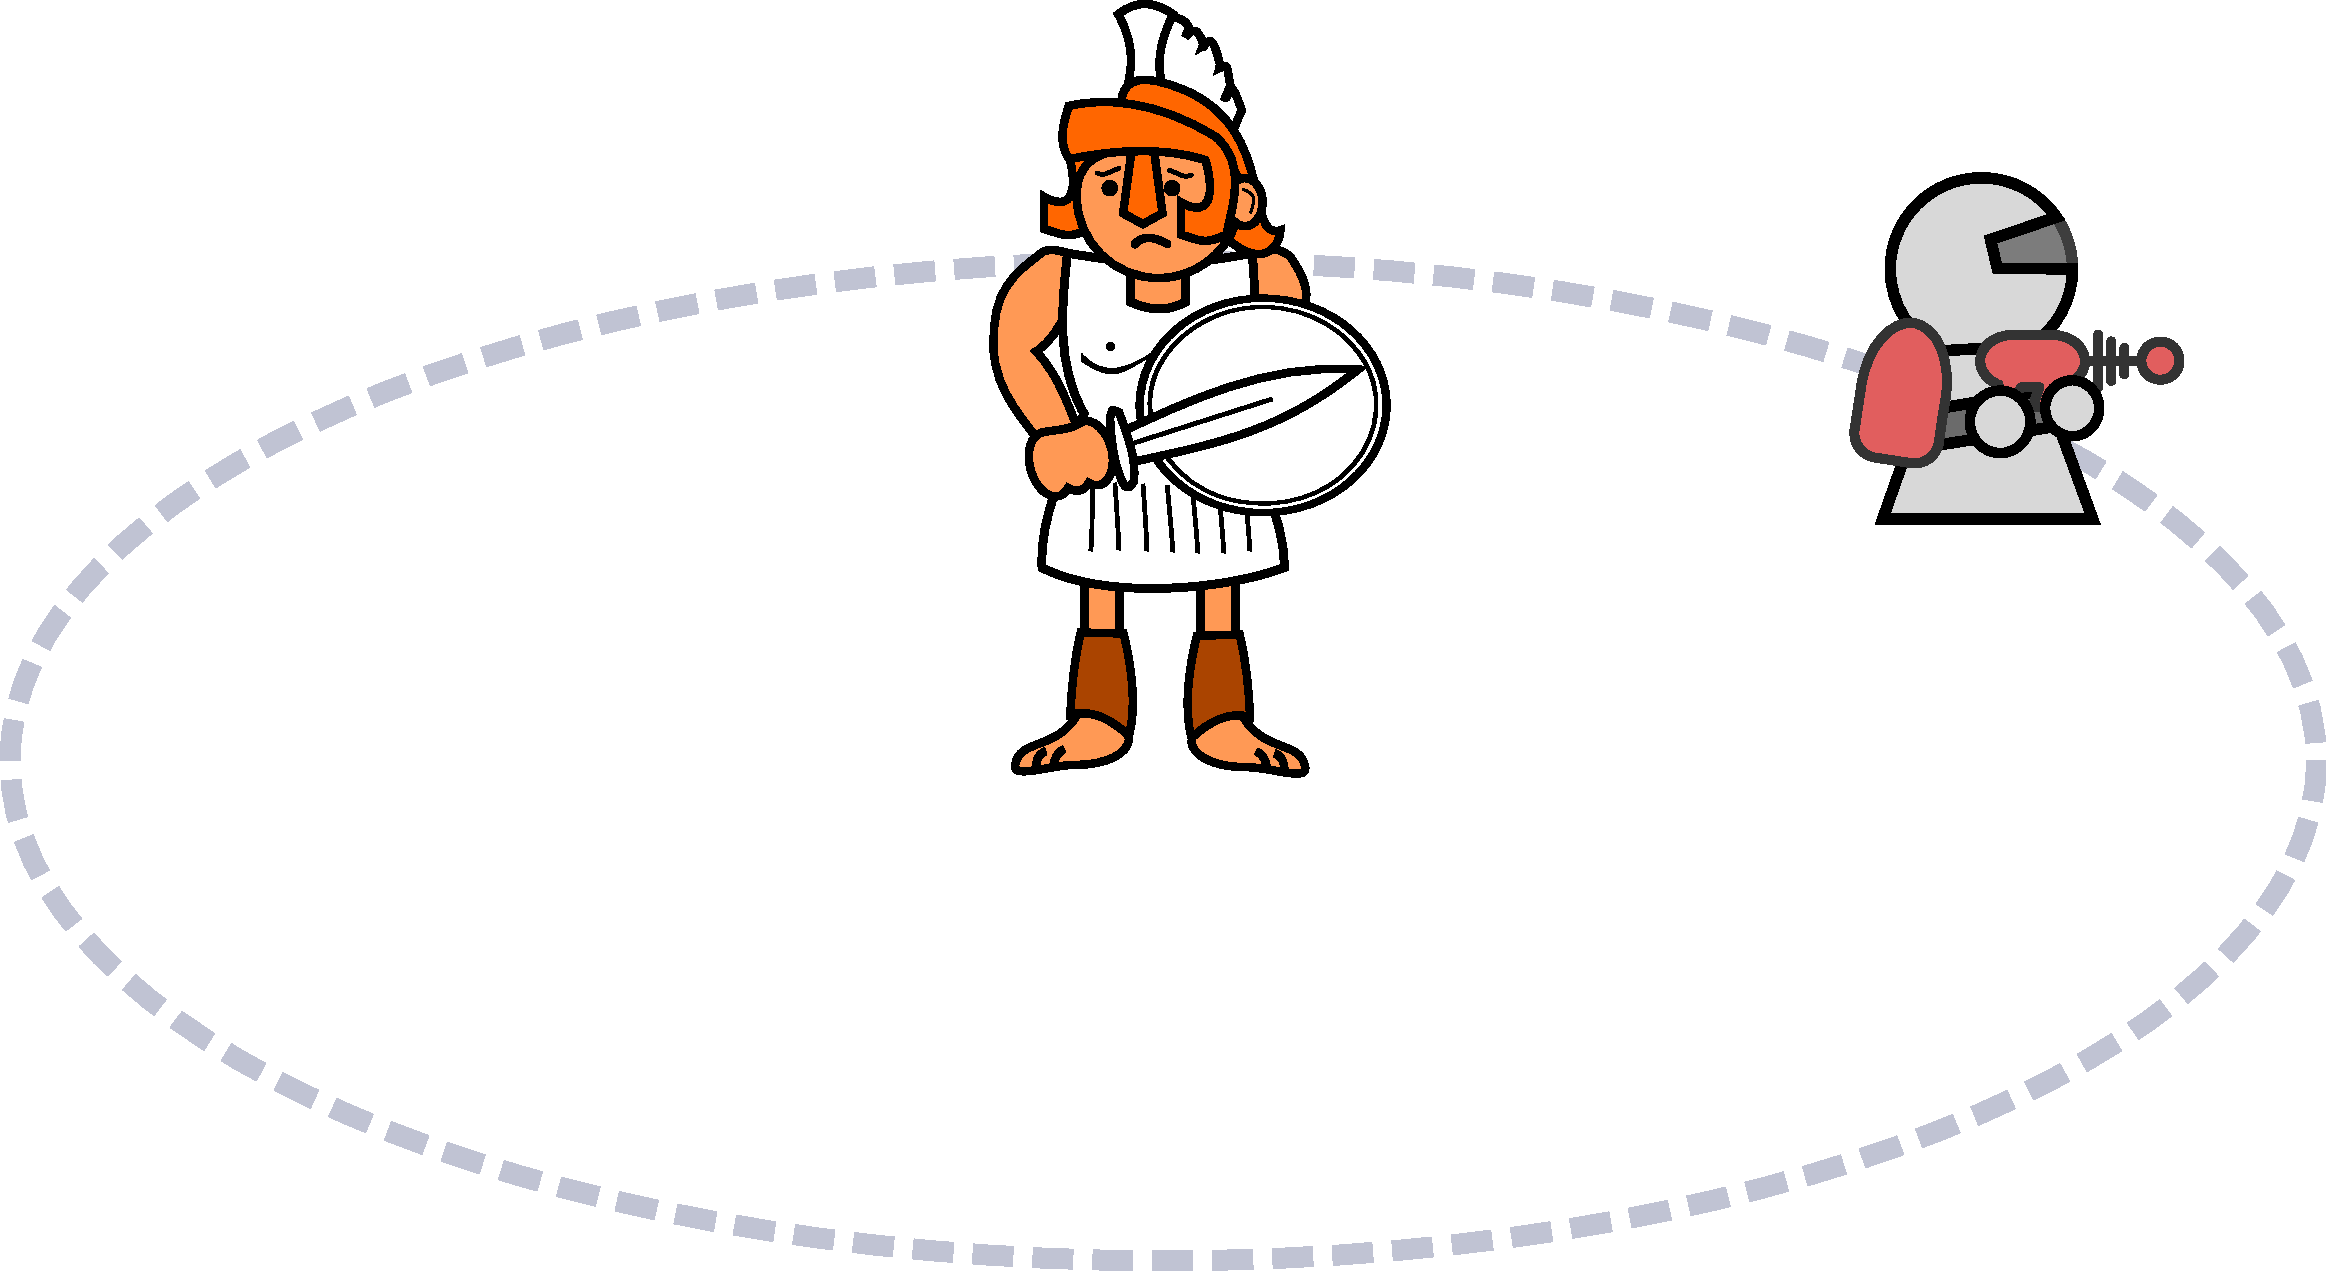
\includegraphics[width = 0.7\textwidth]{./figure/human_robot_interaction}
	\end{figure}
	
	\begin{itemize}
		\item cooperative observation
		\item assistance and protection
	\end{itemize}
	
\end{frame}

\begin{frame}{Neighboring function}{Human constraint}
	\begin{columns}
		\column{.6\linewidth}
		\begin{minipage}[c]{\linewidth}
			\begin{figure}
				\centering
				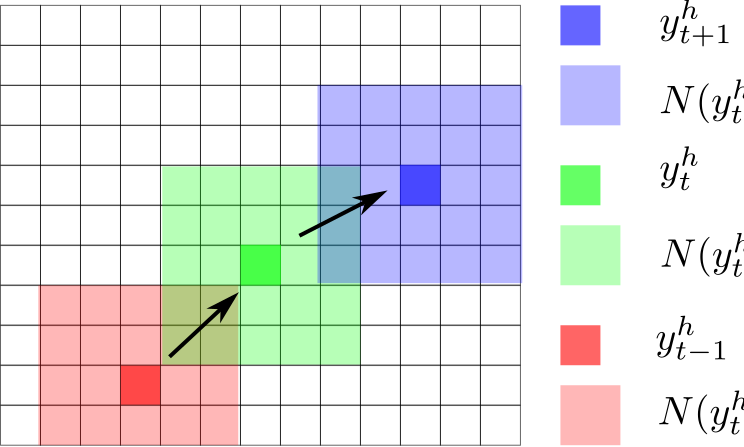
\includegraphics[width = \textwidth]{./figure/humanConstraint}
				%\caption{An example of human constraint.}
			\end{figure}
		\end{minipage}
		
		\column{.4\linewidth}
		\begin{minipage}[c]{\linewidth}
			\begin{itemize}
				\item { human path $ \{ y^{h}_{1} \cdots y^{h}_{T} \} $ }
				\item { neighboring function $ N( y^{h}_{t} ) $ }
			\end{itemize}
		\end{minipage}
	\end{columns}
	
\end{frame}

\begin{frame}{Related work}{ Using a greedy heuristic}
\begin{block}{C.~Chekuri 2005\cite{1530718}}
\begin{itemize}
\item Recursive greedy on a graph topoplogy
\item Edge cost $ \Rightarrow $ Budget 
\end{itemize}
\end{block}
\begin{block}{A.~Singh 2007\cite{singh2007efficient}}
\begin{itemize}
\item Spatial decomposition
\item Recursive greedy of multiple robots
\end{itemize}
\end{block}
\end{frame}

\begin{frame}{Related work}{Using a coarse-to-fine dynamic programming}
\begin{block}{C.~Raphael 2001\cite{Raphael2001}}
Coarse-to-fine backtracking
\end{block}
\begin{figure}
	\centering
	\includegraphics[width = 0.5\textwidth]{./figure/coarse_to_fine_DP}
\end{figure}
\end{frame}






\section{Related Work}
\label{sec:related_work}

If we assume that search targets are static in the search environment, the scan on a location decreases the estimated probability that there is some search target here.
Observations in a search process reduce the uncertainty of where search targets locate.
By measuring this type of uncertainty with information, a search agent can collect more information at non-observed locations than observed ones.
Information gathering is usually selected to measure the efficiency of a search task.
In this paper, we focus on path planning in a search task answers how to maximize information with limited time and resource by defining objective in forms of information evaluation \cite{goodrich2013toward}.

Research work on information maximization path planning focuses a lot on how to solve the optimization problems defined in large scale solution spaces in reasonable time.
\cite{levine2010information} imports ideas of RRT to an information-rich path planning problem, which targets at bringing good efficiency in online optimization in a continuous space.
Under a temporal logic constraint, \cite{JonesSchwagerBeltaICRA13scLTLInfo} use a receding horizon planning to solve an online information-gathering optimization problem.

\begin{figure}
\centering
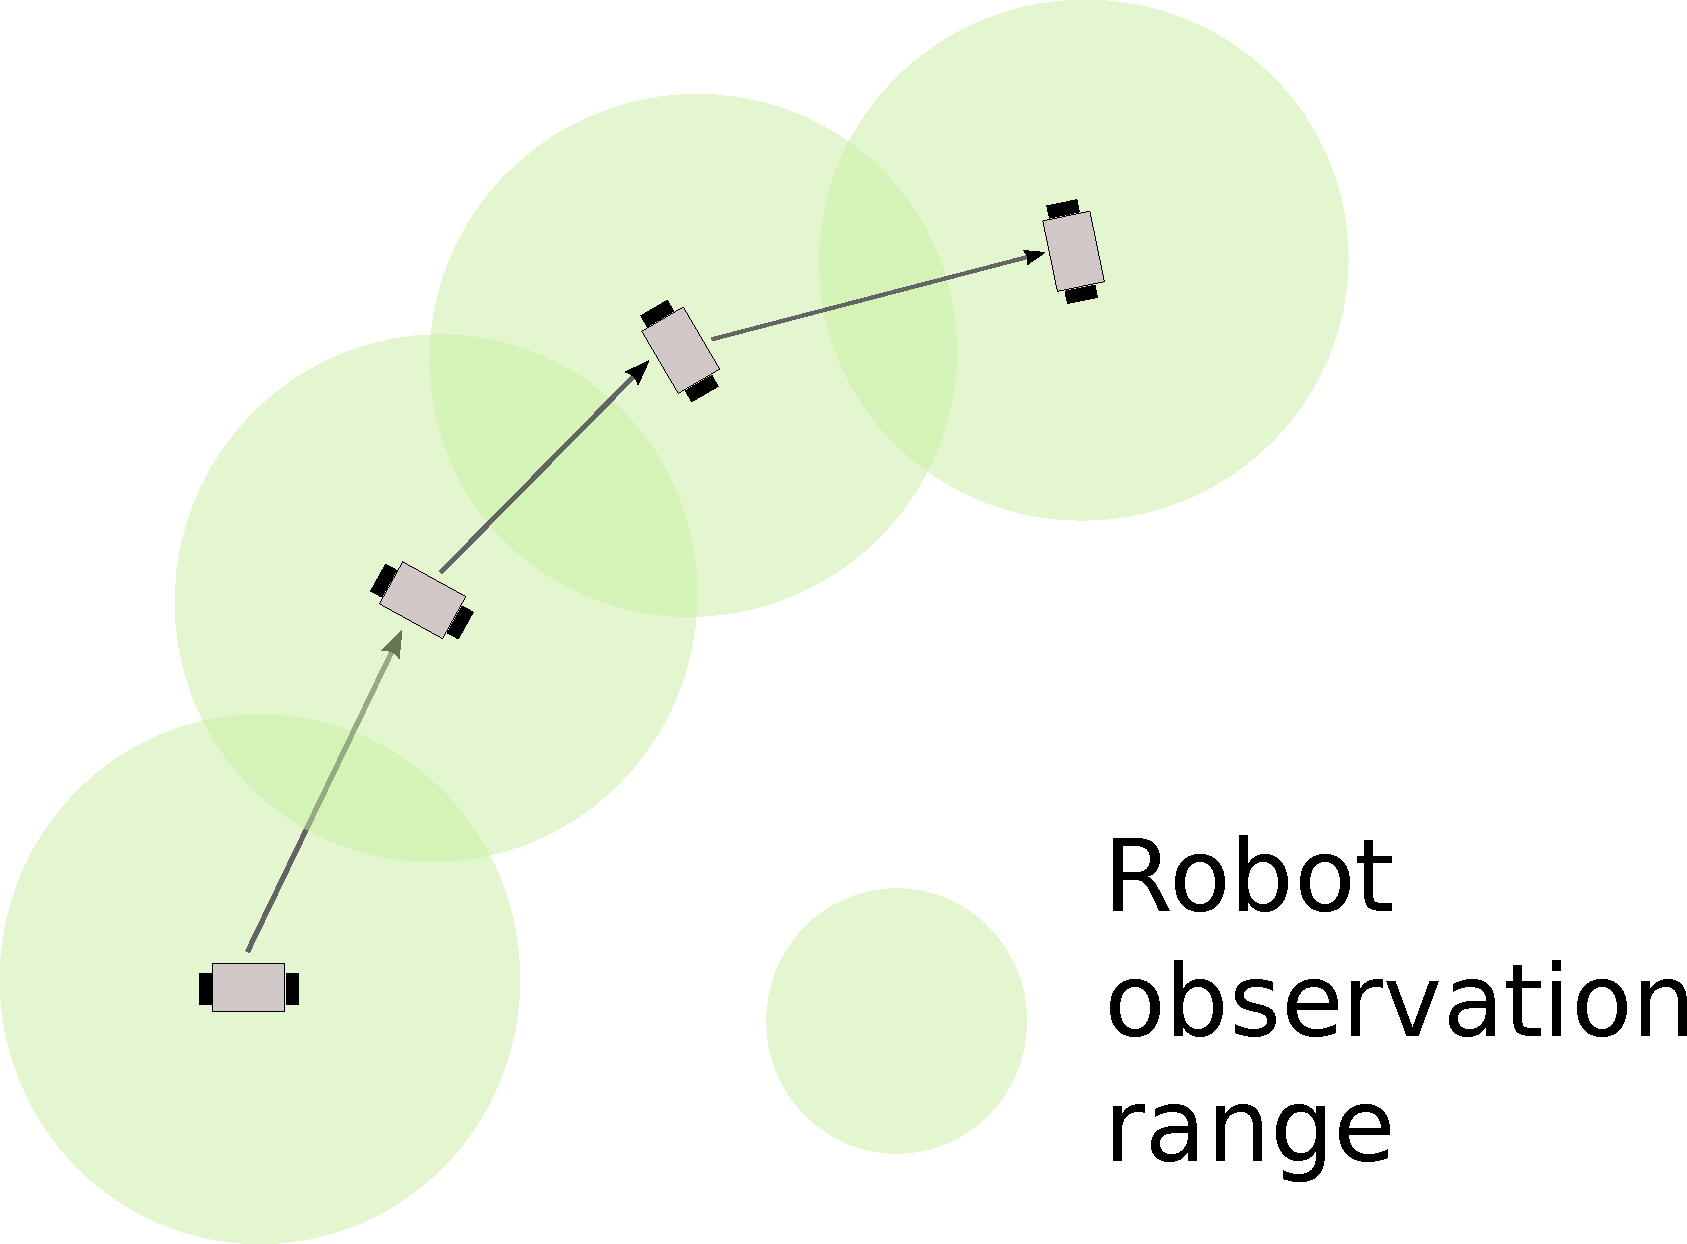
\includegraphics[width=0.4\linewidth]{./images/robotObservation.pdf}
\caption{Maximum coverage in robot observation.}
\label{fig:robotObservation}
\end{figure}

Usually the observation of a search agent covers a much larger region than the area occupied by the robot's body, which is shown in Figure \ref{fig:robotObservation}.
If we consider the observation as a covering range instead of a cell or a point, the overlaps between observation coverage at different time steps must be considered when measuring the total quantity of information.
Figure \ref{fig:robotObservation} gives an example.

Mutual information and conditional mutual information are commonly used to model the overlaps in measuring the total information \cite{singh2009efficient}.
This belongs to a \emph{maximum coverage problem}. 
Multiple sensors placement is one of the applications on information maximization.
In a sequential placement, the locations of placed sensors determine the increase on total information by adding a new sensor.
It is known to be a classical NP-hard combinatorial optimization problem \cite{megiddo1983maximum}.
The problem of maximum coverage on information measurement implies a property of ``nondecreasing submodularity''. 

Maximizing the score collected from a limited-length graph walk is usually known as an \emph{orienteering problem} \cite{Vansteenwegen20111}, in which the total score is a summation of the scores of visited vertices.
If the score function of a vertex has submodularity as in a \emph{maximum coverage problem}, the problem is defined as a \emph{submodular orienteering problem} \cite{chekuri2005recursive}.
A greedy approximation with known performance bound proposed in \cite{singh2009efficient} efficiently exploits the submodularity property of mutual information.
Similarly, in a branch and bound way, \cite{binney2012branch} apply greedy search to informative path planning.
Because the location of the robot at time $ t $ constrains the reachable location at time $ t+1 $, applying greedy algorithm with ``teleport'' assumption to the problem with this constraint can be extremely bad \cite{krause2012submodular}.
In non-teleport motion, \cite{chekuri2005recursive} import recursive greedy by converting to a knapsack constraint so that there is a time resource allocation on planning steps.

Due to the wingman constraint, the path planning of a robot wingman depends on a temporal-space synchronization requirement determined by the positions of a human through time.
The time allocation is fixed and depends on how the human's positions are sampled.
Thus we are not able to model time resource as budget in \cite{chekuri2005recursive}.   

We define the path planning of the robot wingman in a search task as an information maximization problem on a topological graph. We propose an algorithm to solve it as submodular orienteering . The algorithm is designed to produce acceptable robot performance and to be computed efficiently. We then use simulation to demonstrate the acceptable performance of the algorithm and computation efficiency. 


\begin{frame}{$ \null $}{$ \null $}

\centering
{\Large \bf Thank you!}

\end{frame}

\end{document}


